
\section{Desenvolvimento}
	\subsection{FPGA}
	\begin{frame}{Desenvolvimento - FPGA}
		\centering \color{blue} {\Huge \textbf{FPGA} \\[0.5cm]}% {\huge FPGA}
	\end{frame}
	\begin{frame}{Desenvolvimento - FPGA}
		\begin{itemize}
			\item Síntese do algoritmo \textbf{3DES}, no qual utiliza:
			\begin{itemize}
				\item \textbf{Três chaves de 64-\textit{bits}};
				\item \textbf{Blocos de texto de 64-\textit{bits}}.
			\end{itemize}
			\bigskip
			\item Escrita do método de \textbf{envio e recebimento de informações} utilizando protocolo \textbf{UART}\footnote{\textit{\textbf{U}niversal \textbf{A}synchronous \textbf{R}eceiver/\textbf{T}ransmitter}}:
		\end{itemize}
		\begin{figure}[p]
			\centering
			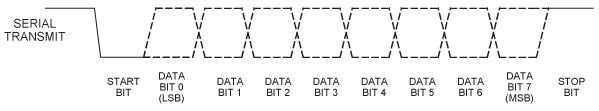
\includegraphics[width=1\textwidth]{img/fpga/uart.png}
			\caption{Protocolo de comunicação UART.}
			\label{fig:uart}
		\end{figure}
	\end{frame}
	\begin{frame}{Desenvolvimento - FPGA - Máquina de Estados Controladora}
		\begin{figure}[p]
			\centering
			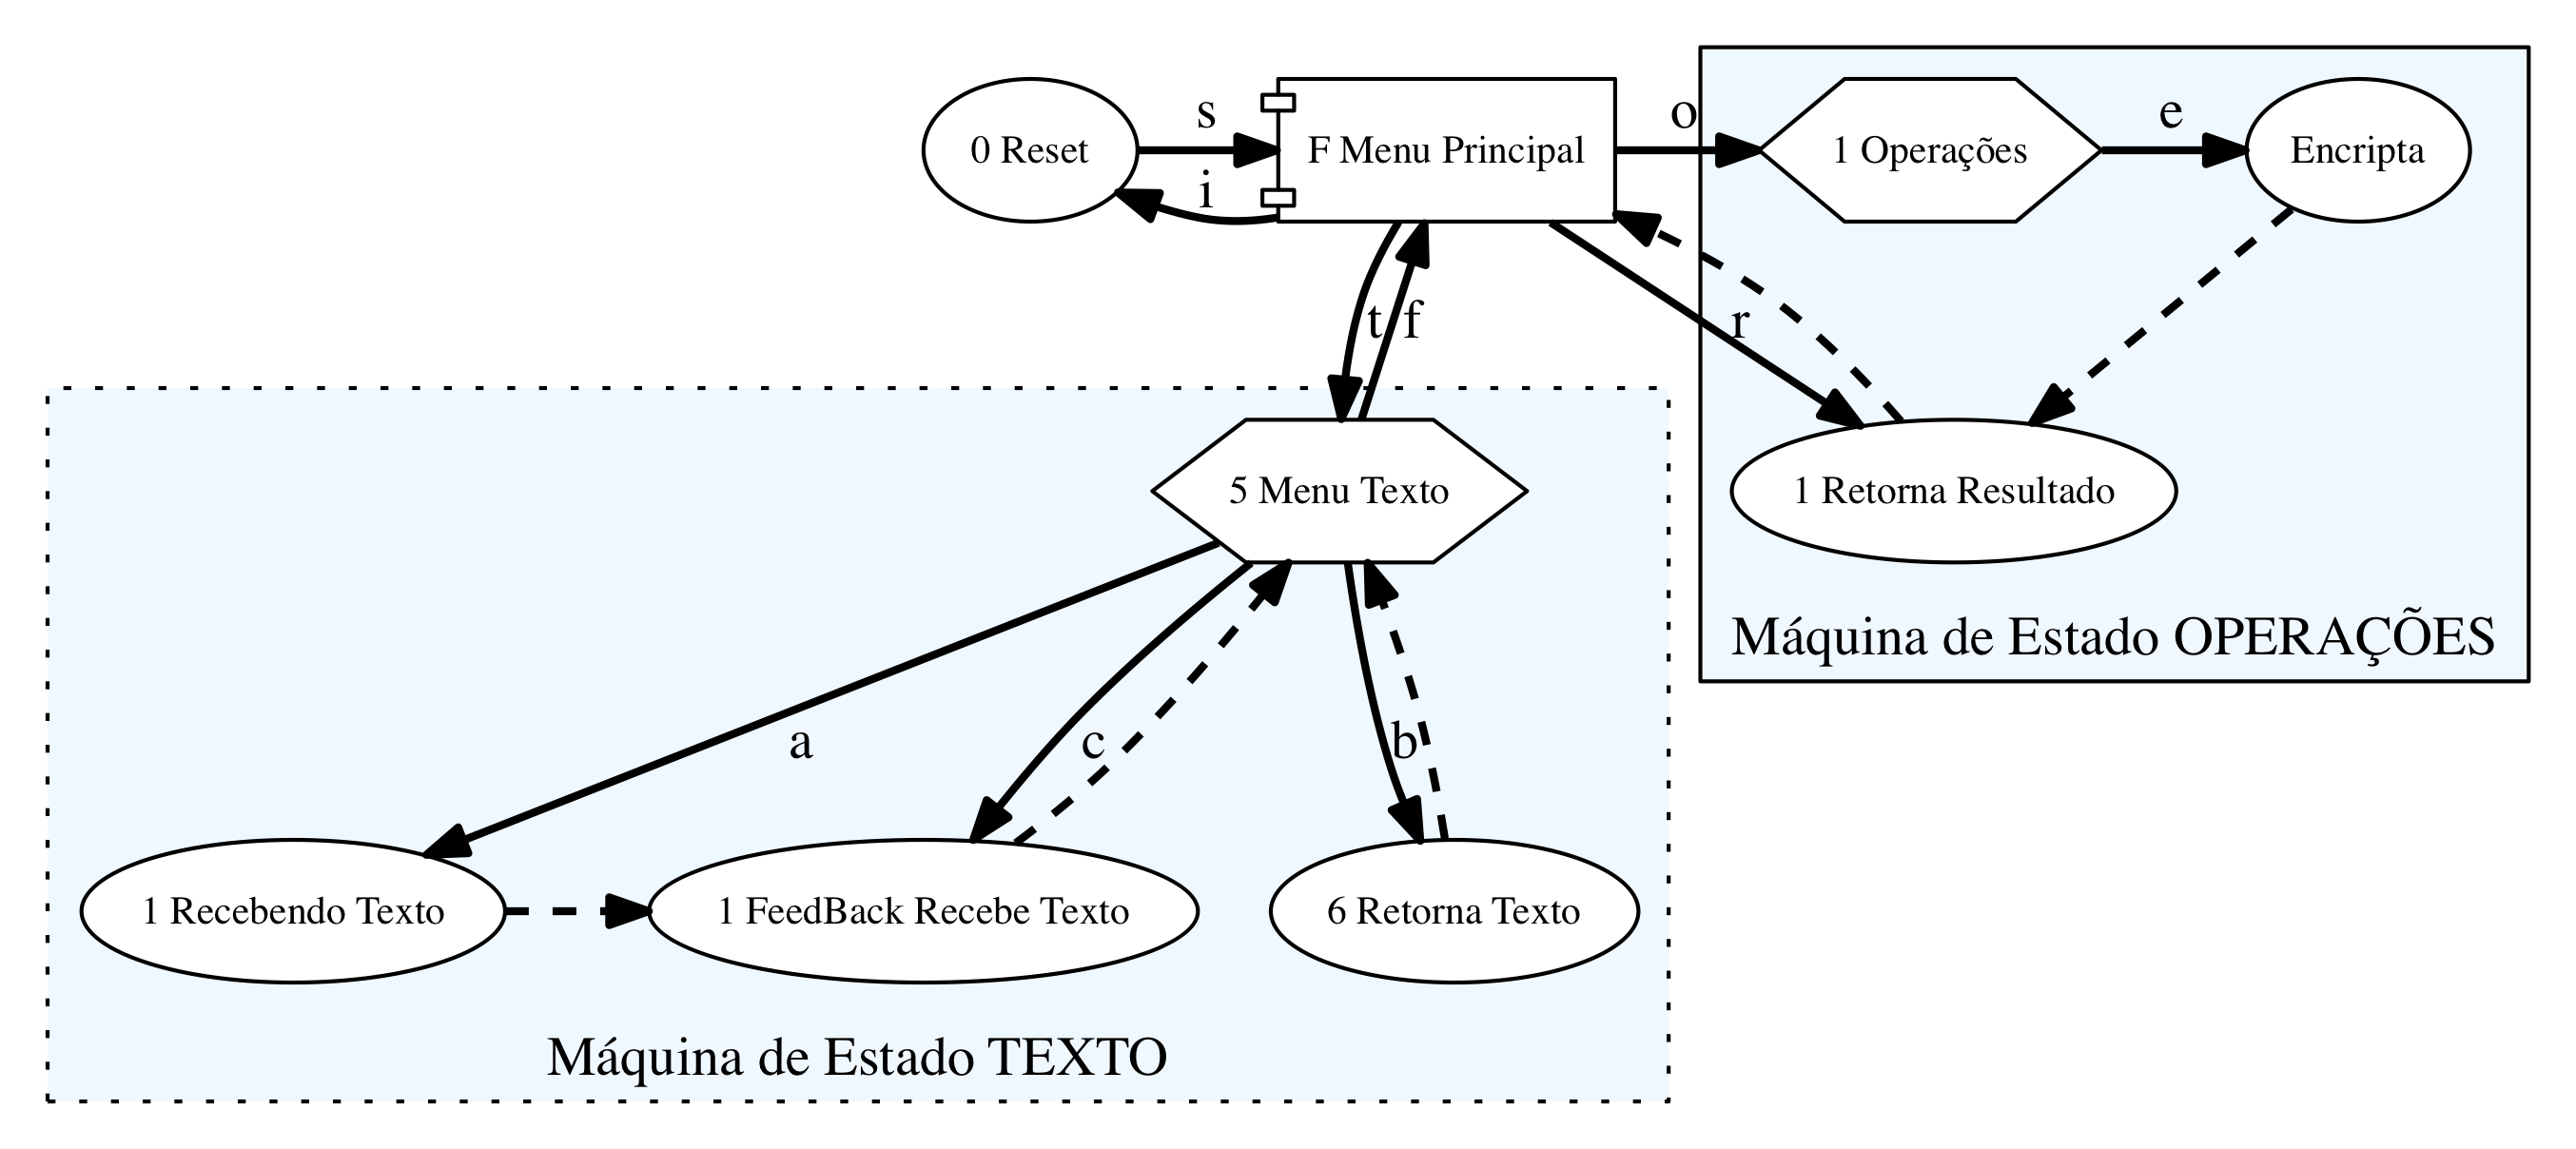
\includegraphics[width=1\textwidth]{img/fpga.png}
			\caption{Exemplo da máquina de Estados do FPGA.}
			\label{fig:mefpga}
		\end{figure}
	\end{frame}


	\subsection{Linux}
	\begin{frame}{Desenvolvimento - Linux}
		\centering \color{blue} {\Huge \textbf{Linux} \\[0.5cm]}
	\end{frame}
	\begin{frame}{Desenvolvimento - Linux}
		\begin{itemize}
			\setlength\itemsep{2em}
			%\item Entendido como compila e carrega um \textit{Driver} ao Kernel, iniciou-se o estudo de desenvolvimento.
			%item Após estudado todas possibilidades de desenvolvimento 
			\item Percebeu-se que existe \textbf{3 classes} de um \textit{Driver} genérico:
			\begin{itemize}
				\setlength\itemsep{1em}
				\item \textbf{Bloco:} 512 \textit{bytes} ou maiores, em potência de 2, mapeado em \texttt{/dev};
				\item \textbf{Interface de Rede:} tratamento de pacote de redes, mapeado como \texttt{eth0};
				\item \textbf{Caractere:} mapeado em \texttt{/dev}.
			\end{itemize}
			\item De todos, o \textit{Driver} pertencentes à classe Caracteres mostrou-se mais \textbf{simples} e \textbf{eficaz} para a comunicação USB.
			%\item Os módulos são desenvolvidos em linguagem C porém com bibliotecas do próprio Kernel.
			%\begin{itemize}
			%	\item \texttt{printf()} por \texttt{printk()};
			%	\item \texttt{malloc()} por \texttt{kalloc()};
			%	\item Entre outros.
			%\end{itemize}
		\end{itemize}
	\end{frame}
	\begin{frame}{Desenvolvimento - Linux}
		\begin{itemize}
			\setlength\itemsep{2em}
			\item Com pesquisas mais profundas, descobriu-se que:
			\begin{itemize}
				\setlength\itemsep{1em}
				\item Unir a comunicação {\bf TTY} (\textit{Driver Char}) com bibliotecas do Kernel específicas para USB torna a escrita mais facilitada;
			\end{itemize}
			%\item Assim, o \textit{Driver} não seria somente um \textit{Driver} de comunicação de caracteres, mas sim com a facilidade do TTY;
			\item Utilizado o TTY com a biblioteca USB Serial:
			\begin{itemize}
				\setlength\itemsep{1em}
				\item Utilizar \textbf{Macros} tornando o processo automatizado;
				\item O \textbf{desenvolvimento} é facilitado;
				\item E consequentemente a \textbf{compreensão}.
			\end{itemize}
			%\item O suporte do \textit{Driver} é descrito numa tabela de dispositivos:
			%\begin{itemize}
			%	\item idVendor, idProduct, ou a classe do dispositivo.
			%\end{itemize}
			%\item Comunicação por meio do diretório \texttt{/dev/tty}
		\end{itemize}
	\end{frame}
	\begin{frame}{Comunicação utilizando TTY}
		%http://www.linusakesson.net/programming/tty/
		\begin{figure}[p]
			\centering
			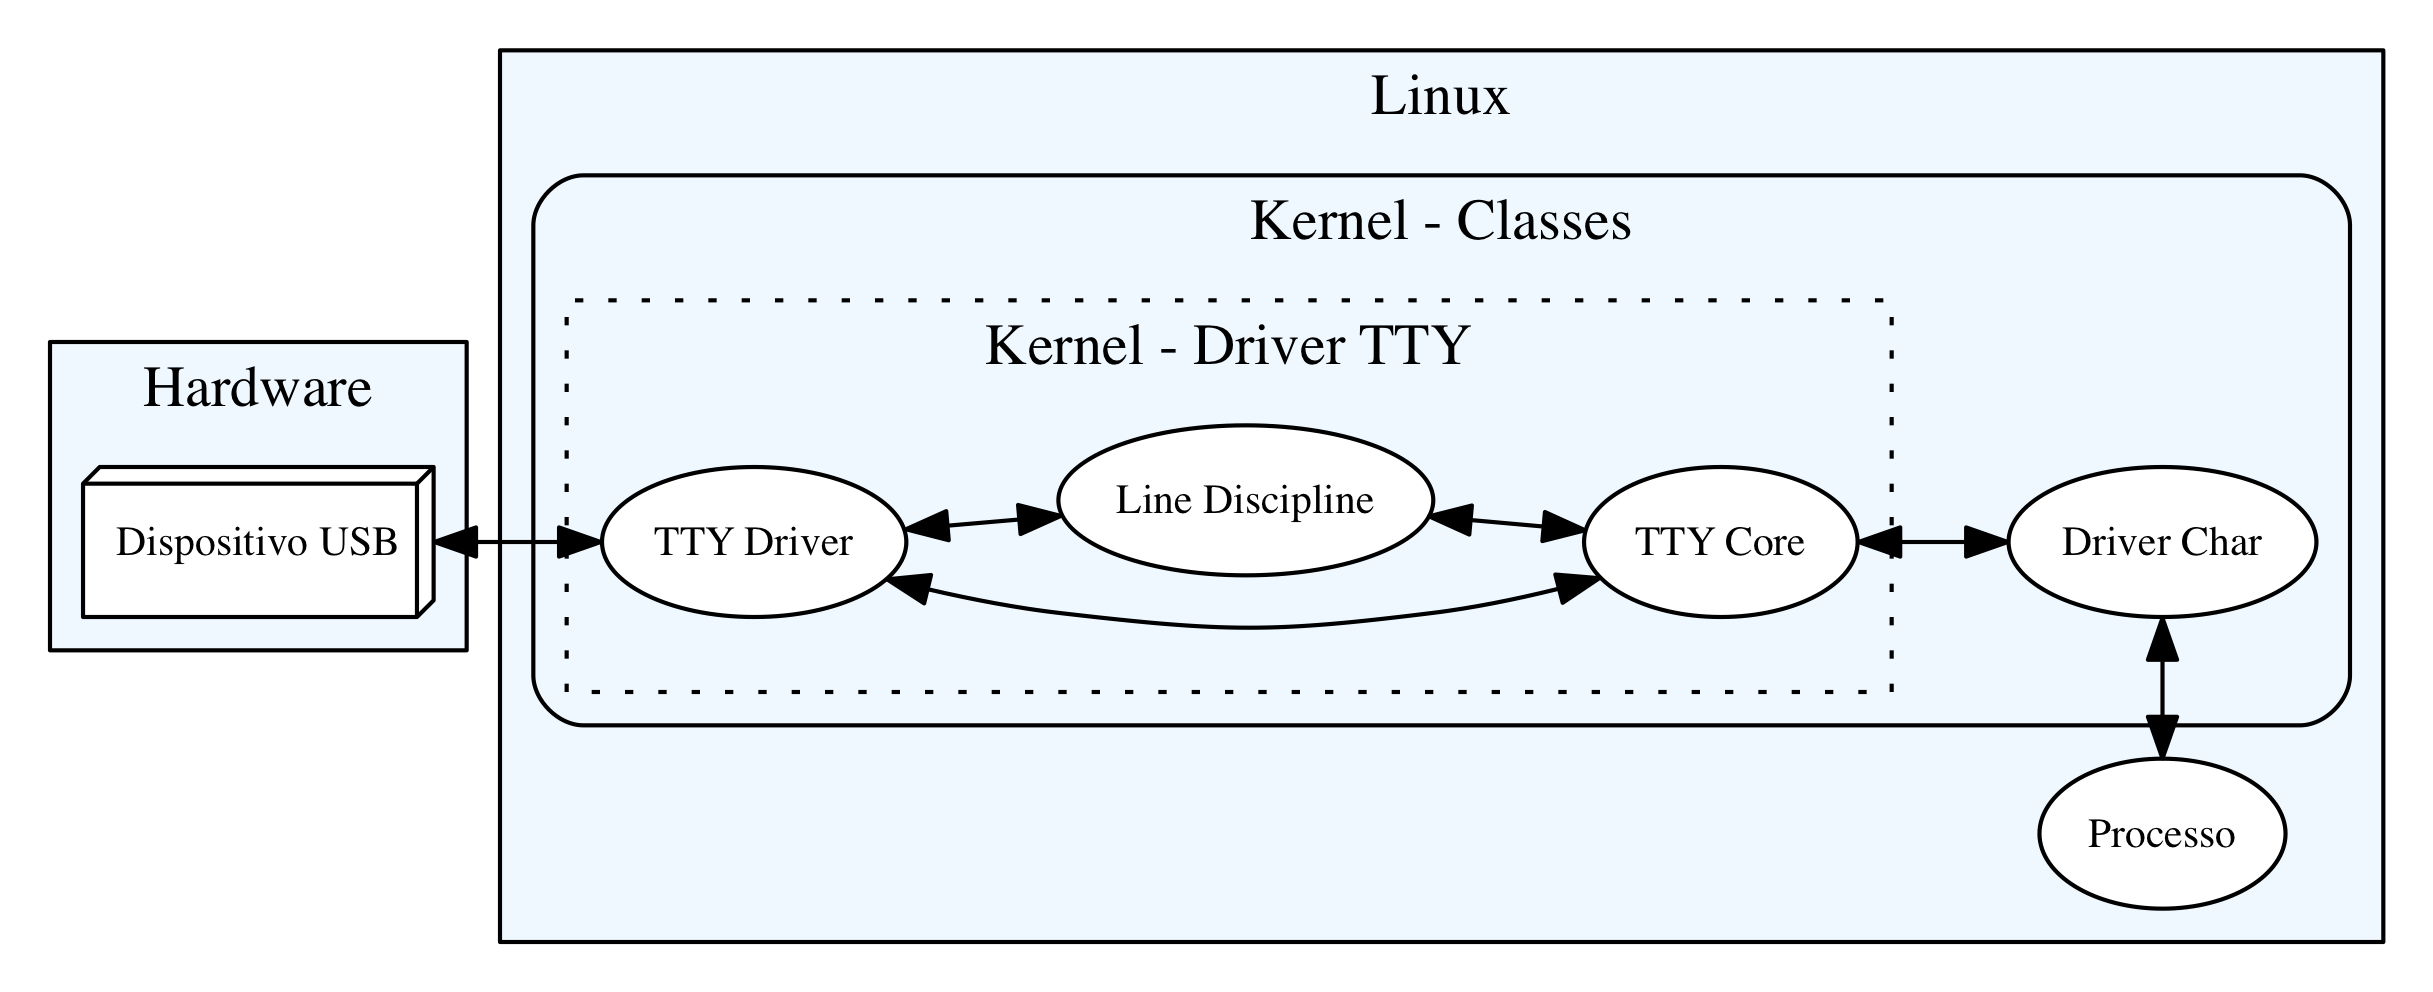
\includegraphics[width=1\textwidth]{img/tty.png}
			\caption{Comunicação utilizando TTY.}
			\label{fig:tty}
		\end{figure}
	\end{frame}


	\subsection{Arduino}
	\begin{frame}{Desenvolvimento - Arduino}
		\centering \color{blue} {\Huge \textbf{Arduino} \\[0.5cm]}
	\end{frame}
	\begin{frame}{Desenvolvimento - Arduino}
		\begin{itemize}
			\setlength\itemsep{2em}
			\item \textbf{Função:} Interconectar o FPGA com o \textit{Driver}.
			\begin{enumerate}
				\setlength\itemsep{1em}
				\item O FPGA não tem interface `\textit{amigável}' para o usuário;
				\item E o \textit{Driver} só realiza a comunicação entre o espaço do usuário com o \textit{hardware}.
			\end{enumerate}
			\item Possui uma máquina de estados no qual:
			\begin{itemize}
				\setlength\itemsep{1em}
				\item \textbf{Controla} as informações a serem exibidas para o usuário;
				\item \textbf{Instrui} quais passos podem ser executados nos momentos certos;
				\item \textbf{Armazena} as informações para operação de forma organizada.
			\end{itemize}
		\end{itemize}
	\end{frame}
	\begin{frame}{Desenvolvimento - Estrutura do Projeto}
		\begin{figure}[p]
			\centering
			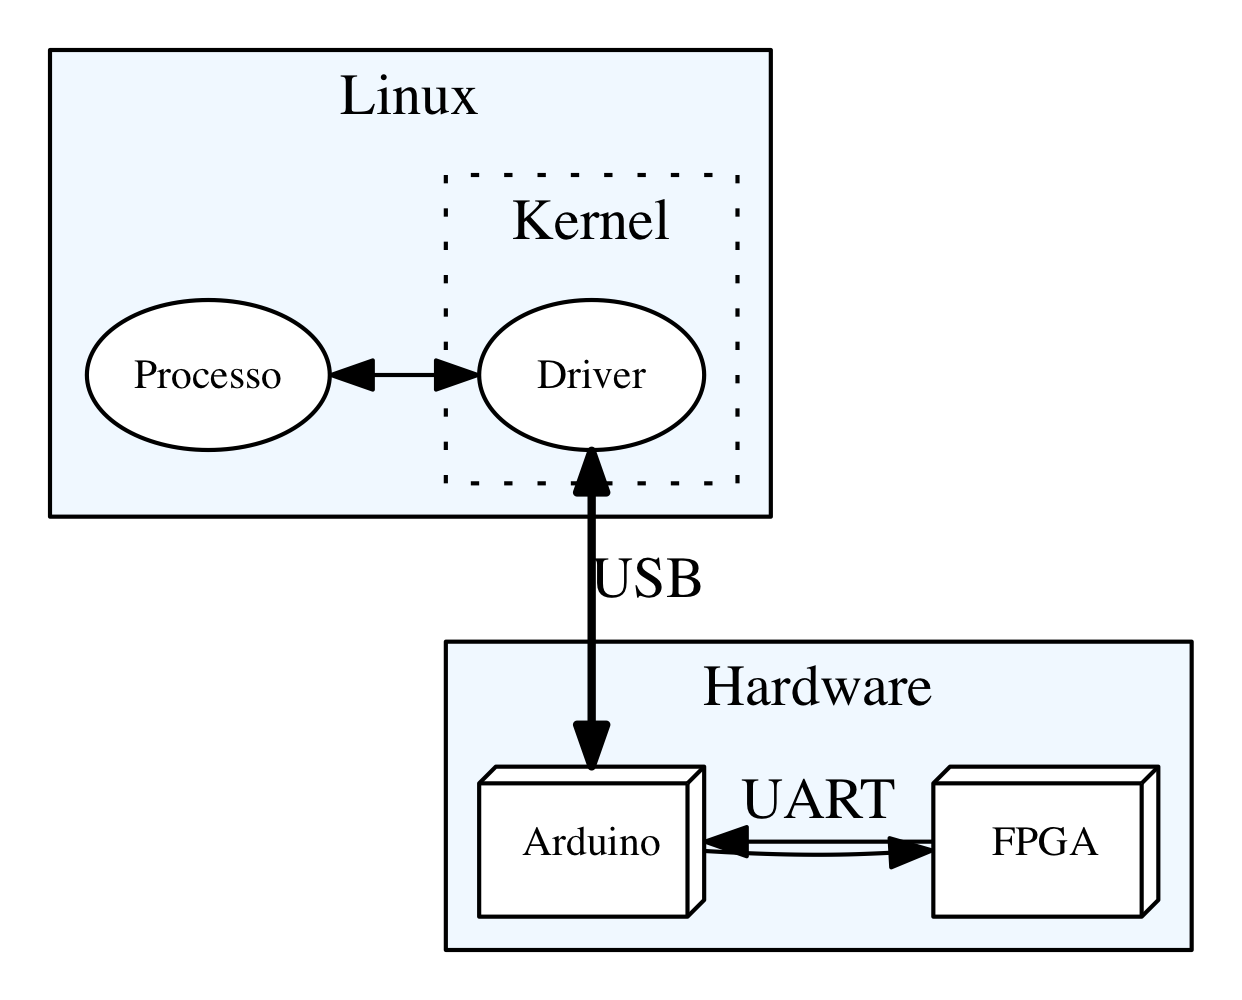
\includegraphics[width=0.72\textwidth]{img/projeto.png}
			\caption{Representação do projeto numa visão geral.}
			\label{fig:projeto}
		\end{figure}
	\end{frame}



%	\begin{frame}{Desenvolvimento - Arduino}
%		\begin{itemize}
%			\item As antigas e as novas (o quão simplificadas elas são em relação às antigas)
%			\item 
%		\end{itemize}
%		\begin{itemize}
%			\item Deixar claro o qur foi feito no FPGA, o que foi feito no Arduino, linguagens utilizadas
%		\end{itemize}
%	\end{frame}

